\documentclass[
  shownotes,
  xcolor={svgnames},
  hyperref={colorlinks,citecolor=DarkBlue,linkcolor=DarkRed,urlcolor=DarkBlue}
  , aspectratio=169]{beamer}
\usepackage{animate}
\usepackage{amsmath}
\usepackage{amsfonts}
\usepackage{amssymb}
\usepackage{pifont}
\usepackage{mathpazo}
%\usepackage{xcolor}
\usepackage{multimedia}
\usepackage{fancybox}
\usepackage[para]{threeparttable}
\usepackage{multirow}
\setcounter{MaxMatrixCols}{30}
\usepackage{subcaption}
\usepackage{graphicx}
\usepackage{lscape}
\usepackage[compatibility=false,font=small]{caption}
\usepackage{booktabs}
\usepackage{ragged2e}
\usepackage{chronosys}
\usepackage{appendixnumberbeamer}
\usepackage{animate}
\setbeamertemplate{caption}[numbered]
\usepackage{color}
%\usepackage{times}
\usepackage{tikz}
\usepackage{comment} %to comment
%% BibTeX settings
\usepackage{natbib}
\bibliographystyle{apalike}
\bibpunct{(}{)}{,}{a}{,}{,}
\setbeamertemplate{bibliography item}{[\theenumiv]}

% Defines columns for bespoke tables
\usepackage{array}
\newcolumntype{L}[1]{>{\raggedright\let\newline\\\arraybackslash\hspace{0pt}}m{#1}}
\newcolumntype{C}[1]{>{\centering\let\newline\\\arraybackslash\hspace{0pt}}m{#1}}
\newcolumntype{R}[1]{>{\raggedleft\let\newline\\\arraybackslash\hspace{0pt}}m{#1}}


\usepackage{xfrac}


\usepackage{multicol}
\setlength{\columnsep}{0.5cm}

% Theme and colors
\usetheme{Boadilla}

% I use steel blue and a custom color palette. This defines it.
\definecolor{andesred}{HTML}{af2433}

% Other options
\providecommand{\U}[1]{\protect\rule{.1in}{.1in}}
\usefonttheme{serif}
\setbeamertemplate{itemize items}[default]
\setbeamertemplate{enumerate items}[square]
\setbeamertemplate{section in toc}[circle]

\makeatletter

\definecolor{mybackground}{HTML}{82CAFA}
\definecolor{myforeground}{HTML}{0000A0}

\setbeamercolor{normal text}{fg=black,bg=white}
\setbeamercolor{alerted text}{fg=red}
\setbeamercolor{example text}{fg=black}

\setbeamercolor{background canvas}{fg=myforeground, bg=white}
\setbeamercolor{background}{fg=myforeground, bg=mybackground}

\setbeamercolor{palette primary}{fg=black, bg=gray!30!white}
\setbeamercolor{palette secondary}{fg=black, bg=gray!20!white}
\setbeamercolor{palette tertiary}{fg=white, bg=andesred}

\setbeamercolor{frametitle}{fg=andesred}
\setbeamercolor{title}{fg=andesred}
\setbeamercolor{block title}{fg=andesred}
\setbeamercolor{itemize item}{fg=andesred}
\setbeamercolor{itemize subitem}{fg=andesred}
\setbeamercolor{itemize subsubitem}{fg=andesred}
\setbeamercolor{enumerate item}{fg=andesred}
\setbeamercolor{item projected}{bg=gray!30!white,fg=andesred}
\setbeamercolor{enumerate subitem}{fg=andesred}
\setbeamercolor{section number projected}{bg=gray!30!white,fg=andesred}
\setbeamercolor{section in toc}{fg=andesred}
\setbeamercolor{caption name}{fg=andesred}
\setbeamercolor{button}{bg=gray!30!white,fg=andesred}


\usepackage{fancyvrb}
\newcommand{\VerbBar}{|}
\newcommand{\VERB}{\Verb[commandchars=\\\{\}]}
\DefineVerbatimEnvironment{Highlighting}{Verbatim}{commandchars=\\\{\}}
% Add ',fontsize=\small' for more characters per line
\usepackage{framed}
\definecolor{shadecolor}{RGB}{248,248,248}
\newenvironment{Shaded}{\begin{snugshade}}{\end{snugshade}}
\newcommand{\AlertTok}[1]{\textcolor[rgb]{0.94,0.16,0.16}{#1}}
\newcommand{\AnnotationTok}[1]{\textcolor[rgb]{0.56,0.35,0.01}{\textbf{\textit{#1}}}}
\newcommand{\AttributeTok}[1]{\textcolor[rgb]{0.77,0.63,0.00}{#1}}
\newcommand{\BaseNTok}[1]{\textcolor[rgb]{0.00,0.00,0.81}{#1}}
\newcommand{\BuiltInTok}[1]{#1}
\newcommand{\CharTok}[1]{\textcolor[rgb]{0.31,0.60,0.02}{#1}}
\newcommand{\CommentTok}[1]{\textcolor[rgb]{0.56,0.35,0.01}{\textit{#1}}}
\newcommand{\CommentVarTok}[1]{\textcolor[rgb]{0.56,0.35,0.01}{\textbf{\textit{#1}}}}
\newcommand{\ConstantTok}[1]{\textcolor[rgb]{0.00,0.00,0.00}{#1}}
\newcommand{\ControlFlowTok}[1]{\textcolor[rgb]{0.13,0.29,0.53}{\textbf{#1}}}
\newcommand{\DataTypeTok}[1]{\textcolor[rgb]{0.13,0.29,0.53}{#1}}
\newcommand{\DecValTok}[1]{\textcolor[rgb]{0.00,0.00,0.81}{#1}}
\newcommand{\DocumentationTok}[1]{\textcolor[rgb]{0.56,0.35,0.01}{\textbf{\textit{#1}}}}
\newcommand{\ErrorTok}[1]{\textcolor[rgb]{0.64,0.00,0.00}{\textbf{#1}}}
\newcommand{\ExtensionTok}[1]{#1}
\newcommand{\FloatTok}[1]{\textcolor[rgb]{0.00,0.00,0.81}{#1}}
\newcommand{\FunctionTok}[1]{\textcolor[rgb]{0.00,0.00,0.00}{#1}}
\newcommand{\ImportTok}[1]{#1}
\newcommand{\InformationTok}[1]{\textcolor[rgb]{0.56,0.35,0.01}{\textbf{\textit{#1}}}}
\newcommand{\KeywordTok}[1]{\textcolor[rgb]{0.13,0.29,0.53}{\textbf{#1}}}
\newcommand{\NormalTok}[1]{#1}
\newcommand{\OperatorTok}[1]{\textcolor[rgb]{0.81,0.36,0.00}{\textbf{#1}}}
\newcommand{\OtherTok}[1]{\textcolor[rgb]{0.56,0.35,0.01}{#1}}
\newcommand{\PreprocessorTok}[1]{\textcolor[rgb]{0.56,0.35,0.01}{\textit{#1}}}
\newcommand{\RegionMarkerTok}[1]{#1}
\newcommand{\SpecialCharTok}[1]{\textcolor[rgb]{0.00,0.00,0.00}{#1}}
\newcommand{\SpecialStringTok}[1]{\textcolor[rgb]{0.31,0.60,0.02}{#1}}
\newcommand{\StringTok}[1]{\textcolor[rgb]{0.31,0.60,0.02}{#1}}
\newcommand{\VariableTok}[1]{\textcolor[rgb]{0.00,0.00,0.00}{#1}}
\newcommand{\VerbatimStringTok}[1]{\textcolor[rgb]{0.31,0.60,0.02}{#1}}
\newcommand{\WarningTok}[1]{\textcolor[rgb]{0.56,0.35,0.01}{\textbf{\textit{#1}}}}
\usepackage{graphicx}
\makeatletter

\definecolor{airforceblue}{rgb}{0.36, 0.54, 0.66}

\usepackage{tikz}
% Tikz settings optimized for causal graphs.
\usetikzlibrary{shapes,decorations,arrows,calc,arrows.meta,fit,positioning}
\tikzset{
    -Latex,auto,node distance =1 cm and 1 cm,semithick,
    state/.style ={ellipse, draw, minimum width = 0.7 cm},
    point/.style = {circle, draw, inner sep=0.04cm,fill,node contents={}},
    bidirected/.style={Latex-Latex,dashed},
    el/.style = {inner sep=2pt, align=left, sloped}
}


\makeatother






%%%%%%%%%%%%%%% BEGINS DOCUMENT %%%%%%%%%%%%%%%%%%

\begin{document}

\title[Lecture 16]{Lecture 16: \\ Linear Model Selection}
\subtitle{Big Data and Machine Learning for Applied Economics \\ Econ 4676}
\date{\today}

\author[Sarmiento-Barbieri]{Ignacio Sarmiento-Barbieri}
\institute[Uniandes]{Universidad de los Andes}


\begin{frame}[noframenumbering]
\maketitle
\end{frame}

%%%%%%%%%%%%%%%%%%%%%%%%%%%%%%%%%%%



%----------------------------------------------------------------------% 

\begin{frame}
\frametitle{Agenda}

\tableofcontents

\end{frame}

%----------------------------------------------------------------------%
\section{Motivation }
\subsection{Recap: Overfit }
%----------------------------------------------------------------------%
\begin{frame}[fragile]
\frametitle{Overfit and out of Sample Prediction}


\begin{itemize}
  \item ML we care about prediction out of sample
  \medskip
  \item Overfit: complex models predict very well inside a sample but "bad" outside
  \medskip
  \item Choose the right complexity level
  \medskip
  \item How do we measure the out of sample error?
  \medskip
  \item $R^2$ doesn't work: measures prediction in sample, it's non decreasing in complexity (PS1)
\end{itemize}

\end{frame}
%----------------------------------------------------------------------%
\begin{frame}[fragile]
\frametitle{Overfit and out of Sample Prediction}


        \begin{figure}[H] \centering
            \captionsetup{justification=centering}
              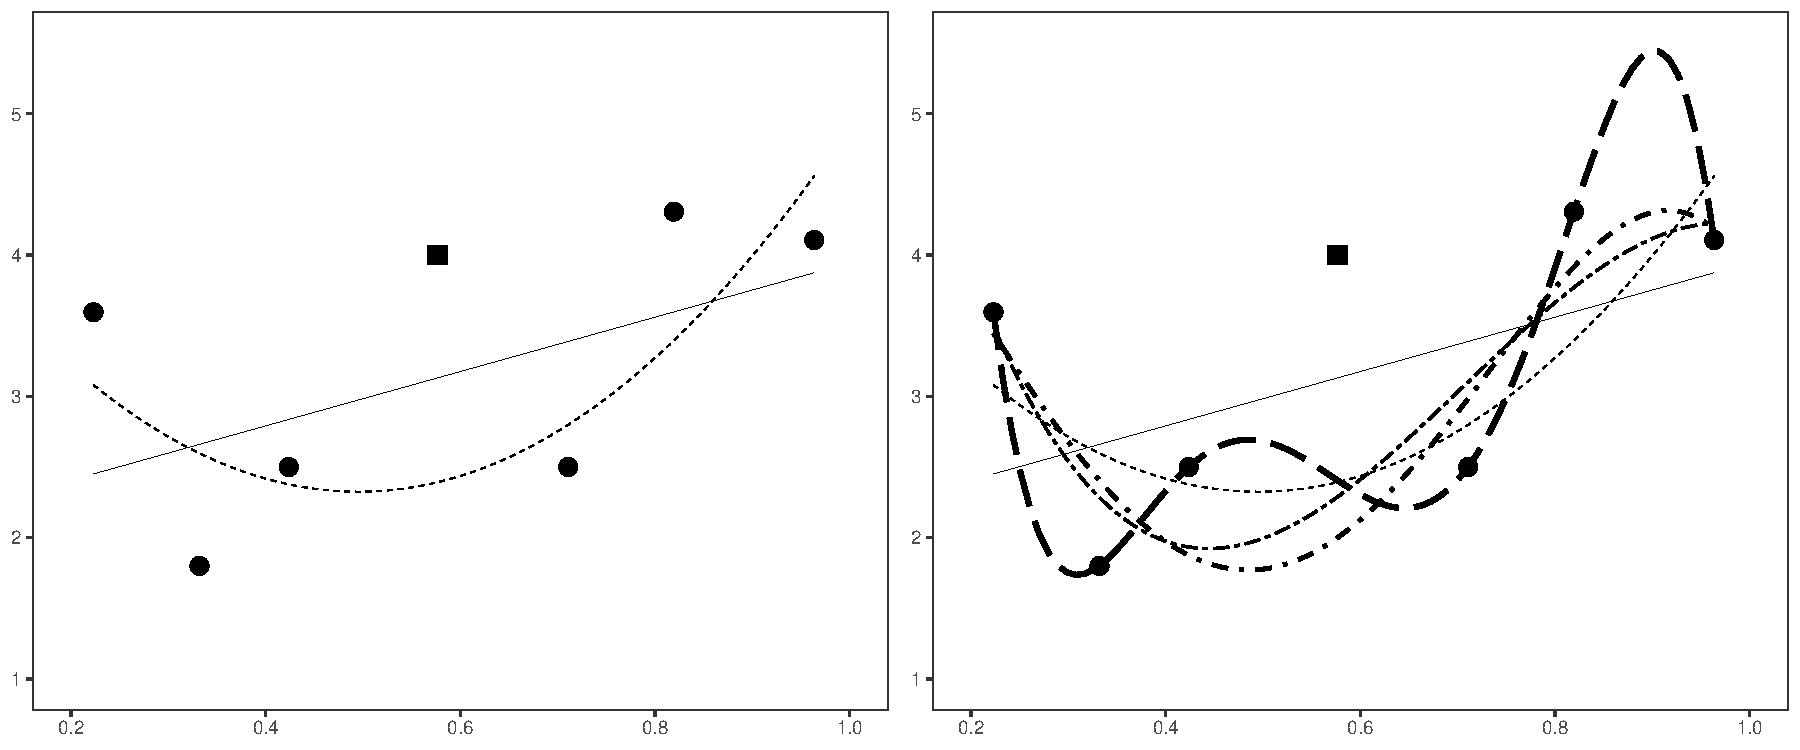
\includegraphics[scale=0.4]{figures/Fig0}
 \end{figure}

\end{frame}
%----------------------------------------------------------------------%
\begin{frame}[fragile]
\frametitle{Motivation}
\begin{itemize}
\item Estimating test error: two approaches
\medskip
\begin{enumerate}
\item We can directly estimate the test error, using either a validation set approach or a cross-validation approach
\medskip
\item We can indirectly estimate test error by making an adjustment to the training error to account for overfitting.
\medskip
\begin{itemize}
  \item AIC, BIC, $C_p$ and Adjusted $R^2$
  \medskip
  \item These techniques adjust the training error for the model size, and can be used to select among a set of models with different numbers of variables.
  \medskip
  \item I'll focus on AIC and BIC. They are intimately related to  more classical notions of hypothesis testing. 
\end{itemize}


\end{enumerate}
\end{itemize}

\end{frame}
%----------------------------------------------------------------------%
\section{Classical Framework for Model Selection}
%----------------------------------------------------------------------%
\begin{frame}[fragile]
\frametitle{Classical Framework for Model Selection }

\begin{itemize}
\item The framework for model selection can be described as follows. 

\item We have a collection of parametric models
\begin{align}
{f_i(x_i,\theta)}
\end{align}

\item where $\theta \in \Theta_j$ for $j = 1,\dots, J$.

 \item Some linear structure is usually imposed on the parameter space, so typically $\Theta_j=m_j\cap\theta_J$ , where $m_j$ is a linear subspace of $\mathcal{R}^{p_J}$ of dimension $p_j$ and $p_1 < p_2 < \dots < p_J$. 
 %\item To formally justify some of our subsequent connections to hypothesis testing it would be also necessary to add the requirement that the models are nested, i.e., that $\Theta_1\subset\Theta_2\subset \dots \Theta_J$
\item e.g.
\begin{align}
y=X_{n\times p_j}\beta+u
\end{align}
\end{itemize}

\end{frame}
%----------------------------------------------------------------------%
\subsection{AIC: Akaike Information Criterion}
%----------------------------------------------------------------------%
\begin{frame}[fragile]
\frametitle{AIC}

\begin{itemize}

\item Akaike (1969) was the first to offer a unified approach to the problem of model selection. 

\item His point of view was to choose a model from the set ${f_i}$ which performed well when evaluated on the basis of forecasting performance. 

\item His criterion, which has come to be called the Akaike information criterion is

\begin{align}
AIC(j) = l_j(\hat \theta) - p_j
\end{align}

\item where $l_j(\theta) $ the log likelihood corresponding to the $j$ model maximized over $\theta\in\Theta_j$. 

\end{itemize}
\end{frame}

%----------------------------------------------------------------------%
\begin{frame}[fragile]
\frametitle{AIC}

\begin{align}
AIC(j) = l_j(\hat \theta) - p_j
\end{align}
\begin{itemize}

\item Akaike’s model selection rule was simply to maximize AIC over the $j$ models, that is to choose the model $j^*$ which maximizes $AIC(j)$.

\item This approach seeks to balance improvement in the fit of the model, as measured by the value of the likelihood, with a penalty term, $p_j$. 

\item Thus one often sees this and related procedures referred to as penalized likelihood methods. 

\item The trade-off is simply: does the improvement which comes inevitably from expanding the dimensionality of the model compensate for the increased penalty?

\end{itemize}
\end{frame}
%----------------------------------------------------------------------%
\subsection{SIC/BIC: Schwarz/Bayesian Information Criterion}
%----------------------------------------------------------------------%
\begin{frame}[fragile]
\frametitle{BIC}
\begin{itemize}
\item Schwarz (1978) showed that while the $AIC$ approach may be quite satisfactory for selecting a forecasting model 
\item However had the unfortunate property that it was inconsistent, in particular, as $n \rightarrow \infty$, it tended to choose too large a model with positive probability. 

\item Schwarz (1978) formalized the model selection problem from a Bayesian standpoint: 
\begin{align}
SIC(j) = l_j(\hat \theta) -\frac{1}{2} p_j log(n)
\end{align}

\item It has the property that as $n\rightarrow \infty$, presuming that there was a true model, $j^*$, then $\hat j =argmax\,\, SIC(j)$, satisfied

\begin{align}
p(\hat j = j^*) \rightarrow 1
\end{align}
\end{itemize}
\end{frame}
%----------------------------------------------------------------------%
\begin{frame}[fragile]
\frametitle{AIC vs BIC}

\begin{align}
AIC(j) = l_j(\hat \theta) - p_j
\end{align}


\begin{align}
SIC(j) = l_j(\hat \theta) -  p_j \frac{1}{2} log(n)
\end{align}

\begin{itemize}
\item Note that  

\begin{align}
\frac{1}{2} log(n) > 1 \,\,\, for \,\,\, n > 8
\end{align}

 \item The SIC penalty is larger than the AIC penalty, 
 \item SIC tends to pick a smaller model. 
 \item In effect, by letting the penalty tend to infinity slowly with n, we eliminate the tendency of AIC to choose too large a model.

\end{itemize}
\end{frame}

%----------------------------------------------------------------------%
\subsection{Connection to Classical Hypothesis Testing: General}
%----------------------------------------------------------------------%
\begin{frame}[fragile]
\frametitle{Connection to Classical Hypothesis Testing: General}
\begin{itemize}
  \item Recall the likelihood ratio tests, that we classically use to assess goodness of fit/ compare models.
  \medskip
  \item Suppose that we are comparing a larger model $j$ to a smaller model $i$
   

   \begin{align}
   T_n=2(l_j(\hat \theta_j)-l_i(\hat \theta_i)) 
   \end{align}
   
  \item It can be shown that $T_n \rightarrow \chi^2_{p_j-p_i}$ for $p_j >p_i=p^*$. 
  \medskip
  \item  So classical hypothesis testing would suggest that we should reject an hypothesized smaller model $i$, in favor of a larger model $j$ iff $T_n$ exceeds an appropriately chosen critical value from the $\chi^2_{p_j-p_i}$ table
\end{itemize}
\end{frame}

 %----------------------------------------------------------------------%
\begin{frame}[fragile]
\frametitle{Connection to AIC}

AIC chooses $j$ over $i$, iff 

\begin{align}
l_j(\hat \theta) - p_j > l_i(\hat \theta) - p_i
\end{align}

\begin{align}
l_j(\hat \theta) - l_i(\hat \theta) > p_j - p_i
\end{align}

\begin{align}
2\frac{l_j(\hat \theta) - l_i(\hat \theta)}{p_j - p_i} > 2
\end{align}

\end{frame}

 %----------------------------------------------------------------------%
\begin{frame}[fragile]
\frametitle{Connection to SIC}

  In contrast Schwarz would choose $j$ over $i$, iff 

 \begin{align}
 \frac{2(l_j(\hat \theta_j)-l_i(\hat \theta_i))}{p_j-p_i} > log(n)
 \end{align}

Then $log(n)$ can be interpreted as an implicit critical value for the model selection decision based on SIC

 \end{frame}

 %----------------------------------------------------------------------%
\subsection{AIC/SIC in the linear regression model}
%----------------------------------------------------------------------%
\begin{frame}[fragile]
\frametitle{AIC/SIC in the linear regression model}
Recall that for the for the Normal/Gaussian linear regression model the log likelihood function is

\begin{align}
l(\beta,\sigma^2) = -\frac{n}{2}log(2\pi)-\frac{n}{2}log(\sigma^2) -\frac{1}{2\sigma^2} (y-X\beta)'(y-X\beta)
\end{align}
evaluating at $\hat \beta$, and $\hat{\sigma}^2=(y-X\hat\beta)'(y-X\hat\beta)$ we get the concentrated/profile log-likelihood

\begin{align}
l(\hat \beta,\hat \sigma^2) = -\frac{n}{2}log(2\pi)-\frac{n}{2}log(\hat \sigma^2) -\frac{n}{2}
\end{align}


 \end{frame}
%----------------------------------------------------------------------%
\begin{frame}[fragile]
\frametitle{AIC/SIC in the linear regression model}
Thus maximizing SIC

\begin{align}
l_i - \frac{1}{2} p_i log(n)
\end{align}

is equivalent to minimize
\begin{align}
\frac{n}{2}log(\hat \sigma_i^2) + \frac{1}{2} p_i log(n)
\end{align}

or minimizing

\begin{align}
log(\hat \sigma_i^2) + \frac{p_i}{n}  log(n)
\end{align}
\begin{itemize}
  \item Similarity for AIC
  \item When using software is important to check what is being computed. In \texttt{R}, the function \texttt{AIC} minimizes and not maximizes, and defines AIC as $-2l_i+kp_i$ with $k=2$ as default that can be changed,e.g. $k=log(n)$ gives SIC
\end{itemize}

 \end{frame}
%----------------------------------------------------------------------%
\begin{frame}[fragile]
\frametitle{Comparison LR, t, AIC, BIC in the linear regression model}

Example of adding one more covariate $p_j-p_i =1$
\begin{align}
T_n=2(l_j(\hat \theta_j)-l_i(\hat \theta_i)) \rightarrow \chi^2_{p_j-p_i}
\end{align}

\begin{align}
\frac{T_n}{p_j-p_i} \rightarrow \frac{\chi^2_{p_j-p_i}}{p_j-p_i}\approx F_{p_j-p_i,\infty}
\end{align}
 \end{frame}
%----------------------------------------------------------------------%
\begin{frame}[fragile]
\frametitle{Comparison LR, t, AIC, BIC in the linear regression model}


\begin{minipage}[t]{0.52\linewidth}
\scriptsize
\begin{align}
\sqrt{2(l_j(\hat \theta_j)-l_i(\hat \theta_i))} \rightarrow \sqrt{F_{1,\infty}}=t_\infty \nonumber
\end{align}

\begin{align}
\sqrt{2 l_j(\hat \theta) - l_i(\hat \theta)} > \sqrt{2} \nonumber
\end{align}

\begin{align}
 \sqrt{2(l_j(\hat \theta_j)-l_i(\hat \theta_i)) }> \sqrt{log(n)} \nonumber
 \end{align}
  \end{minipage}
    \hfill
    \begin{minipage}[t]{0.43\linewidth}%

\begin{figure}[H] \centering
            \captionsetup{justification=centering}
              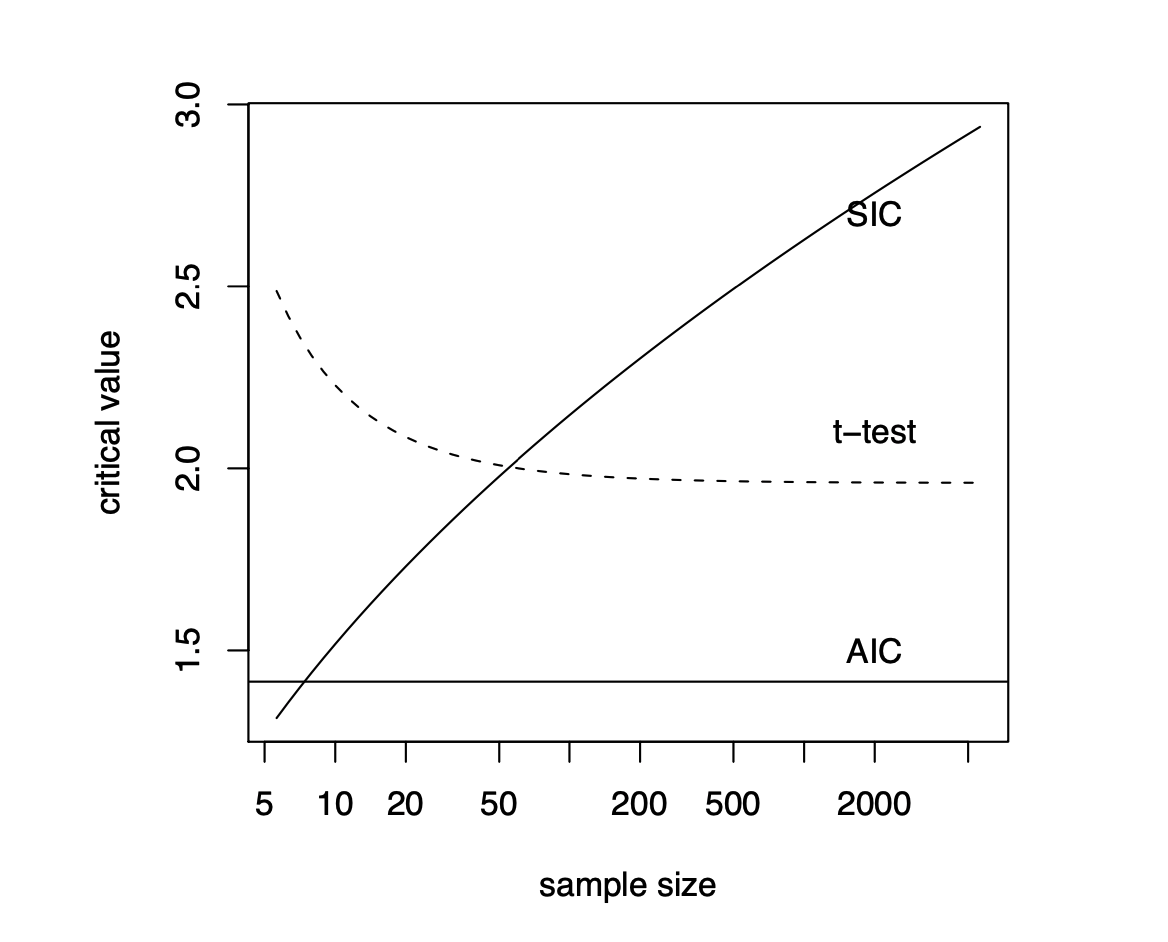
\includegraphics[scale=0.3]{figures/Fig1}
 \end{figure}
   \end{minipage}

\end{frame}
%----------------------------------------------------------------------%
\section{Model Selection in Practice}
%----------------------------------------------------------------------%
\begin{frame}[fragile]
\frametitle{Model Selection in Practice}

\begin{itemize}
\item We have $M_k$ models 
\bigskip
\item We want to find the model that best predicts out of sample
\bigskip
\item We have a number of ways to go about it
\bigskip
\begin{itemize}
  \item Best Subset Selection
  \medskip
  \item Stepwise Selection
  \begin{itemize}
    \item Forward selection
    \medskip
    \item Backward selection
  \end{itemize}
\end{itemize}
\end{itemize}
\end{frame}
%----------------------------------------------------------------------%
\subsection{Best Subset Selection}
%----------------------------------------------------------------------%
\begin{frame}[fragile]
\frametitle{Best Subset Selection}
\begin{enumerate}
\item Let $M_0$ denote the null model, which contains no predictors. This model simply predicts the sample mean for each observation.
\bigskip
\item  For $k=1,2,\dots,p$:
\medskip
\begin{enumerate}
 \item Fit all $\binom{p}{k}$ models that contain exactly k predictors
 \medskip
 \item Pick the best among these $\binom{p}{k}$ models, and call it $M_k$. Where {\it best} is the one with the smallest $SSR$
\end{enumerate}
\bigskip
\item  Select a single best model from among $M_0,\dots, M_p$ using cross-validated prediction error. (ISLR suggest AIC ($C_p$), BIC, or adjusted $R^2$)
\end{enumerate}
 
 \end{frame}

%----------------------------------------------------------------------%
\subsection{Stepwise Selection}
%----------------------------------------------------------------------%
\begin{frame}[fragile]
\frametitle{Stepwise Selection}
 
 \begin{itemize}
\item For computational reasons, best subset selection cannot be applied with very large p. 
\medskip
\item Best subset selection may also suffer from statistical problems when p is large: larger the search space, the higher the chance of finding models that look good on the training data, even though they might not have any predictive power on future data.
\medskip
\item Thus an enormous search space can lead to overfitting and high variance of the coefficient estimates.
\medskip
\item For both of these reasons, stepwise methods, which explore a far more restricted set of models, are attractive alternatives to best subset selection.
\end{itemize}

\end{frame}
%----------------------------------------------------------------------%
\begin{frame}[fragile]
\frametitle{Forward Stepwise Selection}

 \begin{itemize}
\item  Forward stepwise selection begins with a model containing no predictors, and then adds predictors to the model, one-at-a-time, until all of the predictors are in the model.
\bigskip
\item   In particular, at each step the variable that gives the greatest additional improvement to the fit is added to the model.
\end{itemize}

\end{frame}
%----------------------------------------------------------------------%
\begin{frame}[fragile]
\frametitle{Forward Stepwise Selection}

\begin{enumerate}
\item Let $M_0$ denote the null model, which contains no predictors. This model simply predicts the sample mean for each observation.
\bigskip

\item  For $k=0,1,\dots,p-1$:
\medskip
\begin{enumerate}
\item Consider all $p-k$  models that augment the predictors in $M_k$ with one additional predictor.
\medskip
\item Choose the best among these $p - k$ models, and call it $M_{k+1}$. Where {\it best} is the one with the smallest $SSR$
\end{enumerate}
\bigskip
\item Select a single best model from among $M_0,\dots, M_p$ using cross-validated prediction error. (ISLR suggest AIC ($C_p$), BIC, or adjusted $R^2$)
\end{enumerate}

\end{frame}
%----------------------------------------------------------------------%
\begin{frame}[fragile]
\frametitle{Forward Stepwise Selection}


\begin{itemize}
\item Computational advantage over best subset selection is clear.
\item  It is not guaranteed to find the best possible model out of all $2^p$ models containing subsets of the p predictors. 
\item ISLR Example
\end{itemize}

\begin{figure}[H] \centering
            \captionsetup{justification=centering}
              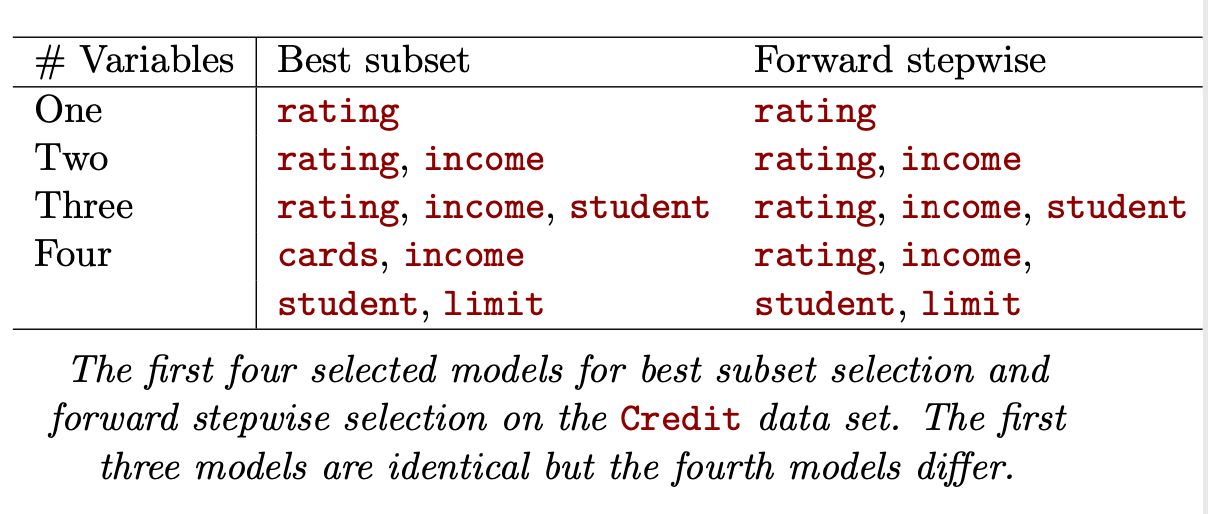
\includegraphics[scale=0.4]{figures/Fig2}
 \end{figure}
\end{frame}
%----------------------------------------------------------------------%
\begin{frame}[fragile]
\frametitle{Backward Stepwise Selection}

\begin{itemize}
\item Like forward stepwise selection, backward stepwise selection provides an efficient alternative to best subset selection.
\bigskip
\item However, unlike forward stepwise selection, it begins with the full least squares model containing all p predictors, and then iteratively removes the least useful predictor, one-at-a-time.
\end{itemize}

\end{frame}
%----------------------------------------------------------------------%
\begin{frame}[fragile]
\frametitle{Backward Stepwise Selection}


\begin{enumerate}
\item Let $M_0$ denote the null model, which contains no predictors. This model simply predicts the sample mean for each observation.
\bigskip

\item  For $k=p,p-1,\dots,1$:
\medskip
\begin{enumerate}
\item Consider all $k$  models that contains all but one of the predictors in $M_k$, for a total of $k-1$ predictors
\medskip
\item Choose the best among these $k$ models, and call it $M_{k-1}$. Where {\it best} is the one with the smallest $SSR$
\end{enumerate}
\bigskip
\item Select a single best model from among $M_0,\dots, M_p$ using cross-validated prediction error. (ISLR suggest AIC ($C_p$), BIC, or adjusted $R^2$)
\end{enumerate}

\end{frame}
%----------------------------------------------------------------------%
\begin{frame}[fragile]
\frametitle{Backward Stepwise Selection}

\begin{itemize}
\item Like forward stepwise selection, the backward selection approach searches through only $1 + p(p + 1)/2$ models, and so can be applied in settings where p is too large to apply best subset selection.
\medskip
\item  Like forward stepwise selection, backward stepwise selection is not guaranteed to yield the best model containing a subset of the p predictors.
\medskip
\item  Backward selection requires that the number of samples n is larger than the number of variables p (so that the full model can be fit). In contrast, forward stepwise can be used even when $n < p$, and so is the only viable subset method when p is very large.
\end{itemize}

\end{frame}
%----------------------------------------------------------------------%
\begin{frame}[fragile]
\frametitle{Validation and Cross-Validation}

\begin{itemize}
\item Each of the procedures returns a sequence of models $M_k$ indexed by model size $k = 0,1,2,\dots$ .
\item Our job here is to select $\hat k$. Once selected, we will return model $M_{\hat{k}}$
\item We compute the validation set error or the cross-validation error for each model $M_k$ under consideration, and then select the $k$ for which the resulting estimated test error is smallest.
\item This procedure has an advantage relative to AIC ($C_p$), BIC, and adjusted $R^2$, in that it provides a direct estimate of the test error, and doesn't require an estimate of the error variance $\sigma^2$
\item It can also be used in a wider range of model selection tasks, even in cases where it is hard to pinpoint the model degrees of freedom (e.g. the number of predictors in the model) or hard to estimate the error variance $\sigma^2$ 
\end{itemize}
\end{frame}


%----------------------------------------------------------------------%
\section{Review \& Next Steps}
%----------------------------------------------------------------------%
\begin{frame}
\frametitle{Review \& Next Steps}
  
\begin{itemize} 
    \item Today:
    \medskip
    \begin{itemize} 
      \item Basic Classical Framework for Model Selection AIC, SIC/BIC
      \medskip
      \item Model Selection in Practice  
        \begin{itemize}  
            \item Best Subset Selection
            \medskip
            \item Stepwise Selection
        \end{itemize}
    \end{itemize}
  	\bigskip  
	\item  Next class after the break:  Regularization/Shrinkage Methods
  \bigskip  
  \item  Remember to work on your proposals

\end{itemize}
\end{frame}

%----------------------------------------------------------------------%
\section{Further Readings}
%----------------------------------------------------------------------%
\begin{frame}
\frametitle{Further Readings}

\begin{itemize}


  \item Friedman, J., Hastie, T., \& Tibshirani, R. (2001). The elements of statistical learning (Vol. 1, No. 10). New York: Springer series in statistics.
  \medskip
  \item James, G., Witten, D., Hastie, T., \& Tibshirani, R. (2013). An introduction to statistical learning (Vol. 112, p. 18). New York: springer.
  \medskip
    \item Koenker, R. (2013) Economics 508: Lecture 4. Model Selection and Fishing for Significance. Mimeo

  
\end{itemize}

\end{frame}

%----------------------------------------------------------------------%
\section{Demo}
%----------------------------------------------------------------------%
\begin{frame}[fragile]
\frametitle{Demo: Prelogomenon}

\begin{scriptsize}
\begin{Shaded}
\begin{Highlighting}[]
\tiny
\CommentTok{\#Load the required packages}
\KeywordTok{library}\NormalTok{(}\StringTok{"McSpatial"}\NormalTok{) }\CommentTok{\#loads the package}
\KeywordTok{library}\NormalTok{(}\StringTok{"dplyr"}\NormalTok{) }\CommentTok{\#for data wrangling}
\KeywordTok{library}\NormalTok{(}\StringTok{"caret"}\NormalTok{) }\CommentTok{\#ML}
\KeywordTok{data}\NormalTok{(matchdata) }\CommentTok{\#loads the data set}
\NormalTok{matchdata \textless{}{-}}\StringTok{ }\NormalTok{matchdata }\OperatorTok{\%\textgreater{}\%}\StringTok{ }\KeywordTok{mutate}\NormalTok{(}\DataTypeTok{price=}\KeywordTok{exp}\NormalTok{(lnprice)) }\OperatorTok{\%\textgreater{}\%}\StringTok{ }\KeywordTok{select}\NormalTok{(}\OperatorTok{{-}}\NormalTok{lnprice) }
\CommentTok{\#transforms log prices to standard prices}
\KeywordTok{set.seed}\NormalTok{(}\DecValTok{123}\NormalTok{) }\CommentTok{\#set the seed for replication purposes}
\KeywordTok{str}\NormalTok{(matchdata) }\CommentTok{\#compact display}
\end{Highlighting}
\end{Shaded}
\end{scriptsize}
\begin{tiny}
\begin{verbatim}
## 'data.frame':    3204 obs. of  18 variables:
##  $ year     : num  1995 1995 1995 2005 1995 ...
##  $ lnland   : num  8.23 8.63 8.7 8.63 8.63 ...
##  $ lnbldg   : num  6.98 7.02 7.22 6.87 7.2 ...
##  $ rooms    : int  5 5 5 4 6 7 7 6 4 6 ...
##  $ bedrooms : int  3 3 3 2 3 3 4 3 2 3 ...
##  $ bathrooms: num  1 1.5 1.5 1 1 2 1 2 1.5 1.5 ...
##  $ centair  : int  0 1 1 0 1 0 1 1 1 1 ...
##  $ fireplace: int  0 0 0 0 0 1 0 0 0 0 ...
##  $ brick    : num  1 1 1 1 1 1 1 1 1 1 ...
##  $ garage1  : num  1 0 0 1 0 1 0 0 1 0 ...
##  $ garage2  : num  0 1 1 0 1 0 1 0 0 0 ...
##  $ dcbd     : num  13.6 13.5 13.6 13.5 13.6 ...
##  $ rr       : num  0 0 0 0 0 0 0 0 0 0 ...
##  $ yrbuilt  : num  1953 1952 1952 1949 1953 ...
##  $ carea    : Factor w/ 11 levels "Albany Park",..: 3 3 3 3 3 3 3 3 3 3 ...
##  $ latitude : num  42 42 42 42 42 ...
##  $ longitude: num  -87.8 -87.8 -87.8 -87.8 -87.8 ...
##  $ price    : num  170750 168000 192500 398000 215000 ...
\end{verbatim}
\end{tiny}

\end{frame}


%----------------------------------------------------------------------%
\begin{frame}[fragile]
\frametitle{Demo: K-fold CV}

\begin{scriptsize}
\begin{Shaded}
\begin{Highlighting}[]
\NormalTok{model2 \textless{}{-}}\StringTok{ }\KeywordTok{train}\NormalTok{(price }\OperatorTok{\textasciitilde{}}\StringTok{ }\NormalTok{bedrooms,   }\CommentTok{\# model to fit}
                     \DataTypeTok{data =}\NormalTok{ matchdata,                        }
                     \DataTypeTok{trControl =} \KeywordTok{trainControl}\NormalTok{(}\DataTypeTok{method =} \StringTok{"cv"}\NormalTok{, }\DataTypeTok{number =} \DecValTok{10}\NormalTok{),     }
                     \CommentTok{\# Method: crossvalidation, 10 folds}
                     \DataTypeTok{method =} \StringTok{"lm"}\NormalTok{)}\CommentTok{\# specifying regression model}

\NormalTok{model2}
\end{Highlighting}
\end{Shaded}
\end{scriptsize}
\begin{tiny}
\begin{verbatim}
## Linear Regression 
## 
## 3204 samples
##    1 predictor
## 
## No pre-processing
## Resampling: Cross-Validated (10 fold) 
## Summary of sample sizes: 2883, 2884, 2884, 2883, 2884, 2885, ... 
## Resampling results:
## 
##   RMSE      Rsquared    MAE     
##   147308.8  0.01385314  122117.8
## 
## Tuning parameter 'intercept' was held constant at a value of TRUE
\end{verbatim}
\end{tiny}
\end{frame}

%----------------------------------------------------------------------%
\begin{frame}[fragile]
\frametitle{Demo: K-fold CV}

\begin{scriptsize}
\begin{Shaded}
\begin{Highlighting}[]
\NormalTok{model2 \textless{}{-}}\StringTok{ }\KeywordTok{train}\NormalTok{(price }\OperatorTok{\textasciitilde{}}\StringTok{ }\NormalTok{bedrooms}\OperatorTok{+}\NormalTok{bathrooms}\OperatorTok{+}\StringTok{ }\NormalTok{rooms}\OperatorTok{+}\NormalTok{centair}\OperatorTok{+}\NormalTok{fireplace}\OperatorTok{+}\NormalTok{brick}\OperatorTok{+}
\StringTok{                        }\NormalTok{lnland}\OperatorTok{+}\NormalTok{lnbldg}\OperatorTok{+}\NormalTok{garage1}\OperatorTok{+}\NormalTok{garage2}\OperatorTok{+}
\StringTok{                        }\NormalTok{dcbd}\OperatorTok{+}\StringTok{ }\NormalTok{rr }\OperatorTok{+}
\StringTok{                        }\NormalTok{yrbuilt}\OperatorTok{+}\StringTok{ }\KeywordTok{factor}\NormalTok{(year) }\OperatorTok{+}
\StringTok{                        }\NormalTok{carea}\OperatorTok{+}\StringTok{ }\NormalTok{latitude}\OperatorTok{+}\NormalTok{longitude,}
                        \DataTypeTok{data =}\NormalTok{ matchdata,                        }
                        \DataTypeTok{trControl =} \KeywordTok{trainControl}\NormalTok{(}\DataTypeTok{method =} \StringTok{"cv"}\NormalTok{, }\DataTypeTok{number =} \DecValTok{10}\NormalTok{), }
                        \DataTypeTok{method =} \StringTok{"lm"}\NormalTok{)}
 
\NormalTok{model2}
\end{Highlighting}
\end{Shaded}
\end{scriptsize}
\begin{tiny}
\begin{verbatim}
## Linear Regression 
## 
## 3204 samples
##   17 predictor
## 
## No pre-processing
## Resampling: Cross-Validated (10 fold) 
## Summary of sample sizes: 2883, 2884, 2884, 2883, 2883, 2884, ... 
## Resampling results:
## 
##   RMSE      Rsquared   MAE     
##   74297.54  0.7490674  48170.37
## 
## Tuning parameter 'intercept' was held constant at a value of TRUE
\end{verbatim}
\end{tiny}

\end{frame}

%----------------------------------------------------------------------%
\frametitle{Model Subset Selection}
%----------------------------------------------------------------------%
\begin{frame}[fragile]
\frametitle{Model Subset Selection}

\begin{itemize}
\item We have $M_k$ models 
\bigskip
\item We want to find the model that best predicts out of sample
\bigskip
\item We have a number of ways to go about it
\bigskip
\begin{itemize}
  \item Best Subset Selection
  \medskip
  \item Stepwise Selection
  \begin{itemize}
    \item Forward selection
    \medskip
    \item Backward selection
  \end{itemize}
\end{itemize}
\end{itemize}
\end{frame}


%----------------------------------------------------------------------%
\begin{frame}[fragile]
\frametitle{Best Subset Selection}
\begin{align}
  y = \beta_0 + \beta_1 X_1 + \dots + \beta_p X_p +u
\end{align}

\begin{enumerate}
\item Estimate {\it \bf all} possible models with $k=0,1,..., p$ predictors.
\bigskip
\item Compute the prediction error using cross validation

\bigskip
\item  Pick the one with the smallest prediction error 
\end{enumerate}

\end{frame}





%----------------------------------------------------------------------%
\begin{frame}[fragile]
\frametitle{Demo: Best Subset Selection}
\begin{itemize}
 \item \texttt{Caret} is usually the solution but it doesn't have everything =(
\end{itemize}
 \begin{figure}[H] \centering
            \captionsetup{justification=centering}
              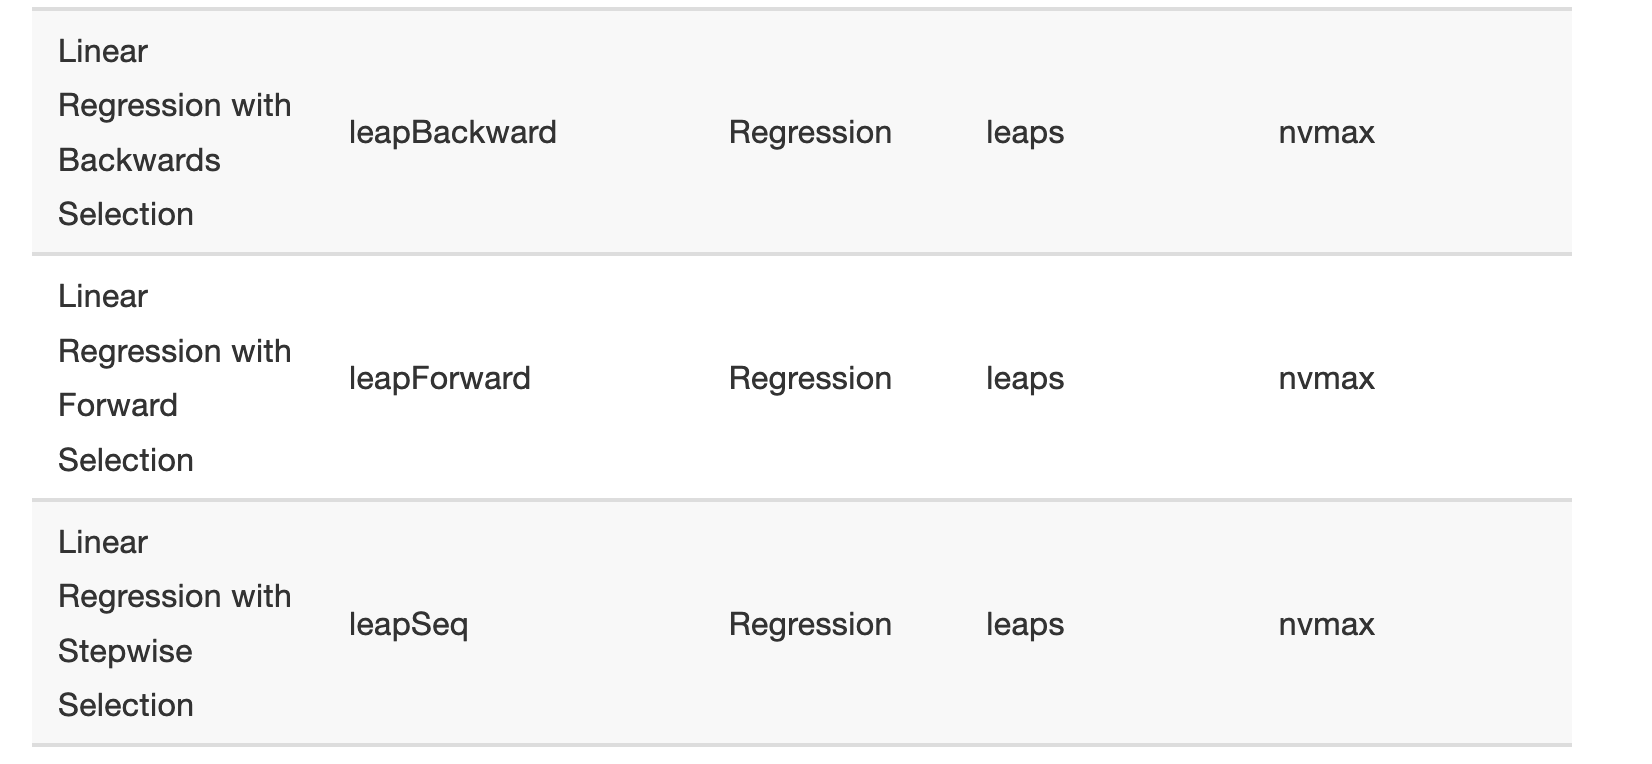
\includegraphics[scale=0.3]{figures/caret_leaps}
\\
\flushleft
              \scriptsize
              Note: \url{https://topepo.github.io/caret/available-models.html}
 \end{figure}


\end{frame}
%----------------------------------------------------------------------%
\begin{frame}[fragile]
\frametitle{Demo: Best Subset Selection}
\begin{Shaded}
\begin{Highlighting}[]
\KeywordTok{require}\NormalTok{(}\StringTok{"leaps"}\NormalTok{)}
\end{Highlighting}
\end{Shaded}

\begin{scriptsize}
\begin{Shaded}
\begin{Highlighting}[]
\KeywordTok{class}\NormalTok{(matchdata}\OperatorTok{$}\NormalTok{carea)}
\end{Highlighting}
\end{Shaded}

\begin{verbatim}
## [1] "factor"
\end{verbatim}

\begin{Shaded}
\begin{Highlighting}[]
\KeywordTok{class}\NormalTok{(matchdata}\OperatorTok{$}\NormalTok{year)}
\end{Highlighting}
\end{Shaded}

\begin{verbatim}
## [1] "numeric"
\end{verbatim}
\begin{Shaded}
\begin{Highlighting}[]
\NormalTok{matchdata}\OperatorTok{$}\NormalTok{year\textless{}{-}}\KeywordTok{factor}\NormalTok{(matchdata}\OperatorTok{$}\NormalTok{year)}
\end{Highlighting}
\end{Shaded}

\begin{Shaded}
\begin{Highlighting}[]
\NormalTok{best\textless{}{-}}\KeywordTok{regsubsets}\NormalTok{(price }\OperatorTok{\textasciitilde{}}\StringTok{ }\NormalTok{., }\DataTypeTok{method=}\StringTok{"exhaustive"}\NormalTok{,}\DataTypeTok{data =}\NormalTok{ matchdata)}
\KeywordTok{summary}\NormalTok{(best)}
\end{Highlighting}
\end{Shaded}
\end{scriptsize}

\end{frame}

%----------------------------------------------------------------------%
\begin{frame}[fragile]
\frametitle{Demo: Best Subset Selection}

\begin{tiny}
\begin{verbatim}
## Subset selection object
## Call: regsubsets.formula(price ~ ., method = "exhaustive", data = matchdata)
## 26 Variables  (and intercept)
## ...
## Selection Algorithm: exhaustive
##          year2005 lnland lnbldg rooms bedrooms bathrooms centair fireplace
## 1  ( 1 ) "*"      " "    " "    " "   " "      " "       " "     " "      
## 2  ( 1 ) "*"      " "    "*"    " "   " "      " "       " "     " "      
## 3  ( 1 ) "*"      "*"    "*"    " "   " "      " "       " "     " "      
## 4  ( 1 ) "*"      "*"    "*"    " "   " "      " "       " "     " "      
## 5  ( 1 ) "*"      "*"    "*"    " "   " "      " "       " "     " "      
## 6  ( 1 ) "*"      "*"    "*"    " "   " "      " "       " "     " "      
## 7  ( 1 ) "*"      "*"    "*"    " "   " "      " "       " "     " "      
## 8  ( 1 ) "*"      "*"    "*"    " "   " "      " "       " "     "*"      
##          brick garage1 garage2 dcbd rr  yrbuilt careaEdgewater careaEdison Park
## 1  ( 1 ) " "   " "     " "     " "  " " " "     " "            " "             
## 2  ( 1 ) " "   " "     " "     " "  " " " "     " "            " "             
## 3  ( 1 ) " "   " "     " "     " "  " " " "     " "            " "             
## 4  ( 1 ) " "   " "     " "     " "  " " " "     "*"            " "             
## 5  ( 1 ) " "   " "     " "     " "  " " " "     "*"            " "             
## 6  ( 1 ) " "   " "     " "     " "  " " " "     "*"            " "             
## 7  ( 1 ) " "   " "     " "     " "  " " " "     "*"            " "             
## 8  ( 1 ) " "   " "     " "     " "  " " " "     "*"            " "      
\end{verbatim}
\end{tiny}
\end{frame}
%----------------------------------------------------------------------%
\begin{frame}[fragile]
\frametitle{Demo: Best Subset Selection}
\begin{tiny}
\begin{verbatim}       
##          careaForest Glen careaJefferson Park careaLincoln Square
## 1  ( 1 ) " "              " "                 " "                
## 2  ( 1 ) " "              " "                 " "                
## 3  ( 1 ) " "              " "                 " "                
## 4  ( 1 ) " "              " "                 " "                
## 5  ( 1 ) "*"              " "                 " "                
## 6  ( 1 ) "*"              " "                 " "                
## 7  ( 1 ) "*"              " "                 "*"                
## 8  ( 1 ) "*"              " "                 "*"                
##          careaNorth Park careaNorwood Park careaRogers Park careaUptown
## 1  ( 1 ) " "             " "               " "              " "        
## 2  ( 1 ) " "             " "               " "              " "        
## 3  ( 1 ) " "             " "               " "              " "        
## 4  ( 1 ) " "             " "               " "              " "        
## 5  ( 1 ) " "             " "               " "              " "        
## 6  ( 1 ) " "             " "               " "              "*"        
## 7  ( 1 ) " "             " "               " "              "*"        
## 8  ( 1 ) " "             " "               " "              "*"        
##          careaWest Ridge latitude longitude
## 1  ( 1 ) " "             " "      " "      
## 2  ( 1 ) " "             " "      " "      
## 3  ( 1 ) " "             " "      " "      
## 4  ( 1 ) " "             " "      " "      
## 5  ( 1 ) " "             " "      " "      
## 6  ( 1 ) " "             " "      " "      
## 7  ( 1 ) " "             " "      " "      
## 8  ( 1 ) " "             " "      " "
\end{verbatim}
\end{tiny}
\end{frame}


%----------------------------------------------------------------------%
\begin{frame}[fragile]
\frametitle{Stepwise Selection}
 
 \begin{enumerate}
 \item Forward Stepwise Selection
 \begin{itemize}
\item Start with no predictors
\medskip
\item Test all models with 1 predictor. Choose the one with smallest prediction error using cross validation
\medskip
\item Add 1 predictor at a time, without taking away. 
\medskip
\item Of the p+1 models, choose the one with smallest prediction error using cross validation
\end{itemize}
\item  Backward Stepwise Selection
\begin{itemize}
  \item Same idea but start with a complete model and go backwards, taking one at a time. 
  \end{itemize}
\end{enumerate}
\end{frame}
%----------------------------------------------------------------------%
\begin{frame}[fragile]
\frametitle{Demo Stepwise Selection}

\begin{scriptsize}
\begin{Shaded}
\begin{Highlighting}[]
\NormalTok{forward \textless{}{-}}\StringTok{ }\KeywordTok{train}\NormalTok{(price }\OperatorTok{\textasciitilde{}}\StringTok{ }\NormalTok{., }\DataTypeTok{data =}\NormalTok{ matchdata,}
              \DataTypeTok{method =} \StringTok{"leapForward"}\NormalTok{,}
              \DataTypeTok{trControl =} \KeywordTok{trainControl}\NormalTok{(}\DataTypeTok{method =} \StringTok{"cv"}\NormalTok{, }\DataTypeTok{number =} \DecValTok{10}\NormalTok{))}
\NormalTok{forward}
\end{Highlighting}
\end{Shaded}
\end{scriptsize}
\begin{tiny}
\begin{verbatim}
## Linear Regression with Forward Selection 
## 
## 3204 samples
##   17 predictor
## 
## No pre-processing
## Resampling: Cross-Validated (10 fold) 
## Summary of sample sizes: 2884, 2884, 2884, 2883, 2883, 2883, ... 
## Resampling results across tuning parameters:
## 
##   nvmax  RMSE      Rsquared   MAE     
##   2      84219.28  0.6768962  55184.58
##   3      79212.49  0.7147519  51009.82
##   4      78595.00  0.7193113  50631.17
## 
## RMSE was used to select the optimal model using the smallest value.
## The final value used for the model was nvmax = 4.
\end{verbatim}
\end{tiny}


\end{frame}
%----------------------------------------------------------------------%
\begin{frame}[fragile]
\frametitle{Demo Stepwise Selection}

\begin{scriptsize}
\begin{Shaded}
\begin{Highlighting}[]
\KeywordTok{summary}\NormalTok{(forward}\OperatorTok{$}\NormalTok{finalModel)}
\end{Highlighting}
\end{Shaded}
\end{scriptsize}
\begin{tiny}
\begin{verbatim}
## Subset selection object
## 26 Variables  (and intercept)
##                     Forced in Forced out
## ...

## 1 subsets of each size up to 4
## Selection Algorithm: forward
##          year2005 lnland lnbldg rooms bedrooms bathrooms centair fireplace
## 1  ( 1 ) "*"      " "    " "    " "   " "      " "       " "     " "      
## 2  ( 1 ) "*"      " "    "*"    " "   " "      " "       " "     " "      
## 3  ( 1 ) "*"      "*"    "*"    " "   " "      " "       " "     " "      
## 4  ( 1 ) "*"      "*"    "*"    " "   " "      " "       " "     " "      
##          brick garage1 garage2 dcbd rr  yrbuilt careaEdgewater careaEdison Park
## 1  ( 1 ) " "   " "     " "     " "  " " " "     " "            " "             
## 2  ( 1 ) " "   " "     " "     " "  " " " "     " "            " "             
## 3  ( 1 ) " "   " "     " "     " "  " " " "     " "            " "             
## 4  ( 1 ) " "   " "     " "     " "  " " " "     "*"            " "             
##          careaForest Glen careaJefferson Park careaLincoln Square
## 1  ( 1 ) " "              " "                 " "                
## 2  ( 1 ) " "              " "                 " "                
## 3  ( 1 ) " "              " "                 " "                
## 4  ( 1 ) " "              " "                 " "                
##          careaNorth Park careaNorwood Park careaRogers Park careaUptown
## 1  ( 1 ) " "             " "               " "              " "        
## 2  ( 1 ) " "             " "               " "              " "        
## 3  ( 1 ) " "             " "               " "              " "        
## 4  ( 1 ) " "             " "               " "              " "        
##          careaWest Ridge latitude longitude
## 1  ( 1 ) " "             " "      " "      
## 2  ( 1 ) " "             " "      " "      
## 3  ( 1 ) " "             " "      " "      
## 4  ( 1 ) " "             " "      " "
\end{verbatim}
\end{tiny}


\end{frame}





%----------------------------------------------------------------------%
\begin{frame}[fragile]
\frametitle{Demo Stepwise Selection}

\begin{scriptsize}
\begin{Shaded}
\begin{Highlighting}[]
\NormalTok{backwards \textless{}{-}}\StringTok{ }\KeywordTok{train}\NormalTok{(price }\OperatorTok{\textasciitilde{}}\StringTok{ }\NormalTok{., }\DataTypeTok{data =}\NormalTok{ matchdata,}
              \DataTypeTok{method =} \StringTok{"leapBackward"}\NormalTok{,}
              \DataTypeTok{trControl =} \KeywordTok{trainControl}\NormalTok{(}\DataTypeTok{method =} \StringTok{"cv"}\NormalTok{, }\DataTypeTok{number =} \DecValTok{10}\NormalTok{))}
\NormalTok{backwards}
\end{Highlighting}
\end{Shaded}
\end{scriptsize}
\begin{tiny}
\begin{verbatim}
## Linear Regression with Backwards Selection 
## 
## 3204 samples
##   17 predictor
## 
## No pre-processing
## Resampling: Cross-Validated (10 fold) 
## Summary of sample sizes: 2884, 2882, 2884, 2885, 2883, 2884, ... 
## Resampling results across tuning parameters:
## 
##   nvmax  RMSE      Rsquared   MAE     
##   2      84353.39  0.6769755  55217.19
##   3      79280.53  0.7153318  51000.22
##   4      78137.63  0.7235894  49820.72
## 
## RMSE was used to select the optimal model using the smallest value.
## The final value used for the model was nvmax = 4.
\end{verbatim}
\end{tiny}
\end{frame}


%----------------------------------------------------------------------%
\begin{frame}[fragile]
\frametitle{Demo Stepwise Selection}

\begin{scriptsize}
\begin{Shaded}
\begin{Highlighting}[]
\KeywordTok{summary}\NormalTok{(backwards}\OperatorTok{$}\NormalTok{finalModel)}
\end{Highlighting}
\end{Shaded}
\end{scriptsize}
\begin{tiny}
\begin{verbatim}
## Subset selection object
## 26 Variables  (and intercept)
## ...
## Selection Algorithm: backward
##          year2005 lnland lnbldg rooms bedrooms bathrooms centair fireplace
## 1  ( 1 ) "*"      " "    " "    " "   " "      " "       " "     " "      
## 2  ( 1 ) "*"      " "    "*"    " "   " "      " "       " "     " "      
## 3  ( 1 ) "*"      "*"    "*"    " "   " "      " "       " "     " "      
## 4  ( 1 ) "*"      "*"    "*"    " "   " "      " "       " "     " "      
##          brick garage1 garage2 dcbd rr  yrbuilt careaEdgewater careaEdison Park
## 1  ( 1 ) " "   " "     " "     " "  " " " "     " "            " "             
## 2  ( 1 ) " "   " "     " "     " "  " " " "     " "            " "             
## 3  ( 1 ) " "   " "     " "     " "  " " " "     " "            " "             
## 4  ( 1 ) " "   " "     " "     " "  " " " "     " "            " "             
##          careaForest Glen careaJefferson Park careaLincoln Square
## 1  ( 1 ) " "              " "                 " "                
## 2  ( 1 ) " "              " "                 " "                
## 3  ( 1 ) " "              " "                 " "                
## 4  ( 1 ) "*"              " "                 " "                
##          careaNorth Park careaNorwood Park careaRogers Park careaUptown
## 1  ( 1 ) " "             " "               " "              " "        
## 2  ( 1 ) " "             " "               " "              " "        
## 3  ( 1 ) " "             " "               " "              " "        
## 4  ( 1 ) " "             " "               " "              " "        
##          careaWest Ridge latitude longitude
## 1  ( 1 ) " "             " "      " "      
## 2  ( 1 ) " "             " "      " "      
## 3  ( 1 ) " "             " "      " "      
## 4  ( 1 ) " "             " "      " "
\end{verbatim}
\end{tiny}

\end{frame}




%----------------------------------------------------------------------%
%----------------------------------------------------------------------%
\end{document}
%----------------------------------------------------------------------%
%----------------------------------------------------------------------%

